\documentclass[11pt]{article}
%\documentclass[conference]{IEEEtran}
%formula
\usepackage{amsmath}
%figure
\usepackage{graphicx}
%table extension
\usepackage{booktabs}
%block diagram
\usepackage{tikz}
\usetikzlibrary{positioning, arrows.meta}
%insert Code
\usepackage{listings}
\usepackage{xcolor}
%symbols
\usepackage{amssymb}
%hyperlink
\usepackage{hyperref}
%auto fig numbering
\usepackage{cleveref}
%micro mod
\usepackage{microtype}

%code view setting
\lstset{
    basicstyle=\ttfamily\small,
    keywordstyle=\color{blue},
    commentstyle=\color{gray},
    numbers=left,
    numberstyle=\tiny,
    frame=single,
    breaklines=true
}

%macro
\newcommand{\R}{\mathbb{R}}
\newcommand{\tf}[2]{\frac{#1}{#2}}

\title{Practice Title}
\author{Youngseok Kim}
%\author{
    %\IEEEauthorblockN{name}
    %\IEEEauthorblockA{affiliation}
%}
\date{\today}

\begin{document}
\maketitle

%section IEEEkeywords

Macro test $\R$.

\section{Practice List}
\begin{itemize}
    \item first
    \item second
\end{itemize}

\begin{enumerate}
    \item one
    \item two
\end{enumerate}

Formula in sentence: $\tau = RC$ RC delay

\begin{equation}
    G(s) = \frac{\omega_n^2}{s^2 + 2\zeta\omega_n s + \omega_n^2}
    %\fraction{zeros}{poles}
    %^{superscript}
    %_{subscript}
    %\sqrt[n]{x} = y <=> y^n = x
    %\alpha \Alpha
    %sigma sum \sum_{k=0}^{n}
    %integral \int_0^\infty
    %differential \dot{x} \ddot{x}
    %package{amsmath}
    %\, thin space
\end{equation}

%difference
Inline: $G(s) = \frac{1}{s + 1}$

Display:
\begin{equation}
    G(s) = \frac{1}{s + 1}
\end{equation}

%matrix
\begin{equation}
%bmatrix []
%pmatrix {}
%vmatrix || (determinant)
%matrix
\begin{bmatrix} 0 & 1 \\ -\frac{k}{m} & -\frac{c}{m}
\end{bmatrix}
\end{equation}

\begin{equation}
%mathbf bold
\dot{\mathbf{x}} =
\begin{bmatrix} 0 & 1 \\ -\frac{k}{m} & -\frac{c}{m} 
\end{bmatrix}
\mathbf{x} +
\begin{bmatrix} 0 \\ \frac{1}{m} \end{bmatrix} u
\end{equation}

Labeling number~\eqref{eq:example}

\begin{equation}
m \ddot{x} + c \dot{x} + k x = u
%labeling
\label{eq:example}
\end{equation}

Figure labeling~\ref{fig:example}

%[ht] here or top
\begin{figure}[ht]
%centering
\centering
%width = 70% of linewidth
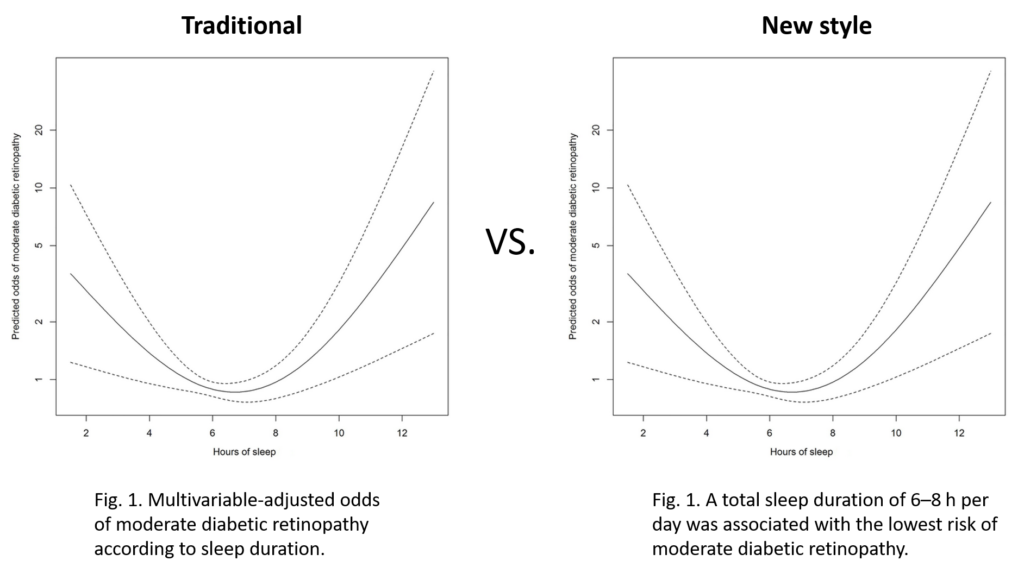
\includegraphics[width=0.7\linewidth]{plot.png}
%caption
\caption{caption.}
\label{fig:example}
\end{figure}

Table labeling~\ref{tab:example}

\begin{table}[ht]
    \centering
    \caption{table}
    \label{tab:example}
    \begin{tabular}{lcc}
        \toprule
        row \\
        \midrule
        1 \\
        2 \\
        3 \\
        \bottomrule
    \end{tabular}
\end{table}

%reference key
Reference~\cite{kalman1960general}

%multiline equation align
\begin{align}
    %align criteria &
    e(t) &= r(t) - y(t)\\
    u(t) &= K_p\, e(t) + K_i \int e(t)\, dt + K_d\, \dot{e}(t)
\end{align}

%separation cases
\begin{equation}
\text{sat}(u) =
\begin{cases}
    u_{\max}, & u > u_{\max} \\
    u,        & |u| \le u_{\max} \\
    u_{\min}, & u < u_{\min}
\end{cases}
\end{equation}

\begin{figure}[ht]
\centering
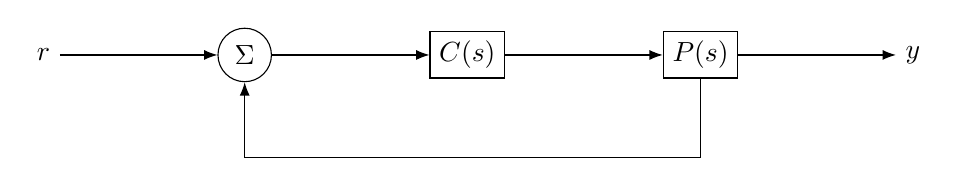
\begin{tikzpicture}[auto, node distance=2cm, >=Latex]
    %\node (name)[option]{content}
    \node (input) {$r$};
    \node (sum) [draw, circle, right=of input] {$\Sigma$};
    \node (ctrl) [draw, right=of sum] {$C(s)$};
    \node (plant) [draw, right=of ctrl] {$P(s)$};
    \node (output) [right=of plant] {$y$};

    \draw[->] (input) -- (sum);
    \draw[->] (sum) -- (ctrl);
    \draw[->] (ctrl) -- (plant);
    \draw[->] (plant) -- (output);
    %feedback
    \draw[->] (plant.south) -- ++(0,-1) -| (sum.south);
\end{tikzpicture}
\caption{caption}
\label{fig:block}

%vertical space 1line
\vspace{1em}

\end{figure}

%insert C code
\begin{lstlisting}[language=C, caption={example}]
void example_function(void* parameters){
    for(int i = 0; i < n; i++)
        parameters->struct_content++;
}
\end{lstlisting}

%reference style
\bibliographystyle{IEEEtran}
%read refs.bib
\bibliography{refs}
\end{document}
